%%%%%%%%%%%%%%%%%%%%%%%%%%%%%%%%%%%%%%%%%%%%%%%%%%%%%%%%%%%%%%%%%%%%%%%%%%%%
% AGUtmpl.tex: this template file is for articles formatted with LaTeX2e,
% Modified July 2014
%
% This template includes commands and instructions
% given in the order necessary to produce a final output that will
% satisfy AGU requirements.
%
% PLEASE DO NOT USE YOUR OWN MACROS
% DO NOT USE \newcommand, \renewcommand, or \def.
%
% FOR FIGURES, DO NOT USE \psfrag or \subfigure.
%
%%%%%%%%%%%%%%%%%%%%%%%%%%%%%%%%%%%%%%%%%%%%%%%%%%%%%%%%%%%%%%%%%%%%%%%%%%%%
%
% All questions should be e-mailed to latex@agu.org.
%
%%%%%%%%%%%%%%%%%%%%%%%%%%%%%%%%%%%%%%%%%%%%%%%%%%%%%%%%%%%%%%%%%%%%%%%%%%%%
%
% Step 1: Set the \documentclass
%
% There are two options for article format: two column (default)
% and draft.
%
% PLEASE USE THE DRAFT OPTION TO SUBMIT YOUR PAPERS.
% The draft option produces double spaced output.
%
% Choose the journal abbreviation for the journal you are
% submitting to:

% jgrga JOURNAL OF GEOPHYSICAL RESEARCH
% gbc   GLOBAL BIOCHEMICAL CYCLES
% grl   GEOPHYSICAL RESEARCH LETTERS
% pal   PALEOCEANOGRAPHY
% ras   RADIO SCIENCE
% rog   REVIEWS OF GEOPHYSICS
% tec   TECTONICS
% wrr   WATER RESOURCES RESEARCH
% gc    GEOCHEMISTRY, GEOPHYSICS, GEOSYSTEMS
% sw    SPACE WEATHER
% ms    JAMES
% ef    EARTH'S FUTURE
% ea    EARTH AND SPACE SCIENCE
%
%
%
% (If you are submitting to a journal other than jgrga,
% substitute the initials of the journal for "jgrga" below.)

%\documentclass[draft,grl]{agutex2015}
\documentclass[grl]{agutex2015}

% To create numbered lines:

% If you don't already have lineno.sty, you can download it from
% http://www.ctan.org/tex-archive/macros/latex/contrib/ednotes/
% (or search the internet for lineno.sty ctan), available at TeX Archive Network (CTAN).
% Take care that you always use the latest version.

% To activate the commands, uncomment \usepackage{lineno}
% and \linenumbers*[1]command, below:

%\usepackage{lineno}
%\linenumbers*[1]
%To add line numbers to lines with equations:
%  \begin{linenomath*}
%  \begin{equation}
%  \end{equation}
%  \end{linenomath*}
%%%%%%%%%%%%%%%%%%%%%%%%%%%%%%%%%%%%%%%%%%%%%%%%%%%%%%%%%%%%%%%%%%%%%%%%%
% Figures and Tables
%
%
% DO NOT USE \psfrag or \subfigure commands.
%
%
%  Uncomment the following command to include .eps files
%  (comment out this line for draft format):
%\usepackage[dvipdf]{graphicx}
\usepackage{graphicx}

% CR added this
\usepackage{color}
\usepackage{amsmath}

%
%  Uncomment the following command to allow illustrations to print
%   when using Draft:
%\setkeys{Gin}{draft=false}
%
% Substitute one of the following for [dvips] above
% if you are using a different driver program and want to
% proof your illustrations on your machine:
%
% [xdvi], [dvipdf], [dvipsone], [dviwindo], [emtex], [dviwin],
% [pctexps],  [pctexwin],  [pctexhp],  [pctex32], [truetex], [tcidvi],
% [oztex], [textures]
%
% See how to enter figures and tables at the end of the article, after
% references.
%
%% ------------------------------------------------------------------------ %%
%
%  ENTER PREAMBLE
%
%% ------------------------------------------------------------------------ %%

% Author names in capital letters:
\authorrunninghead{ROCHA ET AL.}

% Shorter version of title entered in capital letters:
\titlerunninghead{Seasonality at submesoscales}

%Corresponding author mailing address and e-mail address:
\authoraddr{Corresponding author: Cesar B. Rocha,
Scripps Institution of Oceanography, University of California San Diego, La Jolla, CA, USA.
(crocha@ucsd.edu)}

\begin{document}

%% ------------------------------------------------------------------------ %%
%
%  TITLE
%
%% ------------------------------------------------------------------------ %%


\title{Seasonality of submesoscale dynamics in the Kuroshio Extension}
%
% e.g., \title{Terrestrial ring current:
% Origin, formation, and decay $\alpha\beta\Gamma\Delta$}
%

%% ------------------------------------------------------------------------ %%
%
%  AUTHORS AND AFFILIATIONS
%
%% ------------------------------------------------------------------------ %%


%Use \author{\altaffilmark{}} and \altaffiltext{}

% \altaffilmark will produce footnote;
% matching \altaffiltext will appear at bottom of page.

\authors{Cesar B. Rocha\altaffilmark{1}, Sarah T. Gille\altaffilmark{1},
        Teresa K. Chereskin\altaffilmark{1}, and Dimitris Menemenlis\altaffilmark{2}}
% Eric Brown,\altaffilmark{1,2} Rick Williams,\altaffilmark{3}
% John B. McDougall\altaffilmark{4}, and S. Visconti\altaffilmark{5}}

\altaffiltext{1}{Scripps Institution of Oceanography, University of California San Diego, La Jolla, CA, USA.}
\altaffiltext{2}{Earth Sciences Division, Jet Propulsion Laboratory, California Institute of Technology, Pasadena, CA, USA.}


%\altaffiltext{2}{Department of Geography, Ohio State University,
%Columbus, Ohio, USA.}

%\altaffiltext{3}{Department of Space Sciences, University of
%Michigan, Ann Arbor, Michigan, USA.}

%\altaffiltext{4}{Division of Hydrologic Sciences, Desert Research
%Institute, Reno, Nevada, USA.}

%\altaffiltext{5}{Dipartimento di Idraulica, Trasporti ed
%Infrastrutture Civili, Politecnico di Torino, Turin, Italy.}

%% ------------------------------------------------------------------------ %%
%
%  KEYPOINTS
%
%% ------------------------------------------------------------------------ %%

% Key points are 1 to 3 points that the author provides,
% that are 100 characters or less, that are ultimately published
% with the article.
%% for example:
% \keypoints{\item Here is the first keypoint. what happens if it is a
% long keypoint, like this one. We want to see this wrap please.
% \item This is the second.
% \item And here is the third keypoint
% }

\keypoints{\item  Upper-ocean submesoscale (10-100 km) turbulence and inertia-gravity waves
                  undergo strong seasonal cycles that are out of phase.
           \item  Submesoscale turbulence dominates the horizontal velocity and
                  sea-surface height variability in late winter/early spring.
            \item Submesoscale inertia-gravity waves dominate the horizontal velocity and
                   sea-surface height variability in late summer/early fall.
                  }

%% Keypoints will print underneath the abstract.


%% ------------------------------------------------------------------------ %%
%
%  ABSTRACT
%
%% ------------------------------------------------------------------------ %%

% >> Do NOT include any \begin...\end commands within
% >> the body of the abstract.

\begin{abstract}
    Two new high-resolution numerical simulations with embedded tides show a
    strong modulation of near-surface dynamics at submesoscales
    (roughly 10-100 km) in the Kuroshio Extension. Consistent with recent studies, deep late-winter mixed layers
    are prone to baroclinic instabilities, and submesoscale turbulence
    prevails in late winter/early spring. While summertime
    re-stratification weakens submesoscale turbulence, it also enhances submesoscale inertia-gravity
     waves near the surface. In the Kuroshio Extension,
    inertia-gravity waves strongly dominate the submesoscale surface kinetic energy and
    sea-surface height variance in late summer/early fall.
\end{abstract}

%% ------------------------------------------------------------------------ %%
%
%  BEGIN ARTICLE
%
%% ------------------------------------------------------------------------ %%

% The body of the article must start with a \begin{article} command
%
% \end{article} must follow the references section, before the figures
%  and tables.

\begin{article}

%% ------------------------------------------------------------------------ %%
%
%  TEXT
%
%% ------------------------------------------------------------------------ %%

\section{Introduction}

Recent interest in upper-ocean dynamics has focused on the strong seasonal
cycle of shallow baroclinic instabilities and their role in submesoscale (roughly 1-100 km)
turbulence and mesoscale (roughly 100-300 km) modulation \citep{sasaki_etal2014,qiu_etal2014,
callies_etal2015, thompson_etal2016,buckingham_etal2016}. Contemporary studies
have also shown that inertia-gravity waves contribute significantly
to the near-surface variability at submesoscales \citep{richman_etal2012,
buhler_etal2014,rocha_etal2016}, but their seasonality has not been investigated.

Using the output of $1/24^\circ$ and $1/48^\circ$ global
numerical simulations with embedded tides, we show that inertia-gravity waves undergo
a strong seasonality near the surface in the Kuroshio Extension region.
Interestingly, the seasonal cycle of inertia-gravity waves is out of phase
with the seasonal cycle of submesoscale turbulence. On one hand, consistent with previous studies,
deep late-winter mixed layers are prone to
shallow baroclinic instabilities that are roughly in geostrophic balance
and flux energy upscale \citep{sasaki_etal2014,callies_etal2016},
driving a mild seasonal modulation of the mesoscales \citep{sasaki_etal2014,qiu_etal2014}.

Inertia-gravity waves, on the other hand, peak in late summer/early fall,
when the upper ocean is strongly stratified. Thus there exists a
strong seasonal modulation of upper-ocean submesoscale dynamics:
submesoscale turbulence dominates the upper-ocean dynamics in late winter/early fall,
whereas submesoscale inertia-gravity waves prevail in late summer/early fall.
Because submesoscale turbulence is weakest in late summer/early fall,
the present results indicate that inertia-gravity waves account for most of the
summertime submesoscale sea-surface height variability.

\section{The LLC numerical simulations}
We use results of two latitude-longitude polar cap (LLC)
realistic numerical simulations. The outputs
analyzed here, LLC2160 (1/24$^\circ$) and LLC4320 (1/48$^\circ$),   are
forward Massachusetts Institute of Technology general circulation model \citep[MITgcm; ][]{marshall_etal1997}
numerical solutions on a LLC grid  \citep{forget_etal2015} with
90-vertical-levels. The coarser-resolution LLC simulation was
spun up from an Estimating the Circulation and Climate of the Ocean, Phase II \citep[ECCO2; ][]{menemenlis_etal2008}
adjoint-method state estimate, constrained to millions
of observations from 2009 through 2011. Both simulations were forced by
tides hourly and by 6-hourly surface atmospheric fields. The LLC2160
output spans two years from March 2011 to April 2013; the LLC4320 was spun up from
the LLC2160 simulation, spanning one year from September 2011 to October 2012.
The LLC4320 simulation is an extension of the 3-month long output used by
\citet{rocha_etal2016}.  Details of the LLC simulations are provided in the supplemental material.

A key aspect of the LLC2160 and LLC4320 simulations is that they were forced by
the 16 most-significant tidal components.
Because barotropic tides interact with topography and generate internal
tides that project onto mesoscales to submesoscales
\citep[e.g., ][]{rocha_etal2016}, tidal forcing fundamentally distinguishes our analysis
from other modeling studies of seasonality \citep{sasaki_etal2014,qiu_etal2014}.

To study seasonal variations in the upper-ocean dynamics, we focus on the northwest
Pacific, in the vicinity of the Kuroshio
Extension, where previous studies have shown strong mesoscale and submesoscale seasonality
\citep{sasaki_etal2014,qiu_etal2014}.
We analyze a sub-domain of the LLC4320 and LLC2160 simulations of about 2000 km$^2$
spanning 155-175$^\circ$E; 25-40$^\circ$N (Figure \ref{fig1}a). The stratification
in this mesoscale-rich subtropical region undergoes a vigorous seasonal cycle: wintertime-enhanced
small-scale turbulence de-stratifies the upper ocean, yielding mixed layers
as deep as 300 m (Figure \ref{fig1}d). Summertime re-stratification yields mixed layers shallower
than 40 m (Figure \ref{fig1}e).
Fundamentally, the upper-ocean density structure is well-captured by both LLC simulations:
a comparison with Argo climatology shows that both simulations skillfully represent the Kuroshio
Extension stratification and its seasonal variability  (supporting information).

\begin{figure*}[ht]
\begin{center}
\hspace{-1.25cm}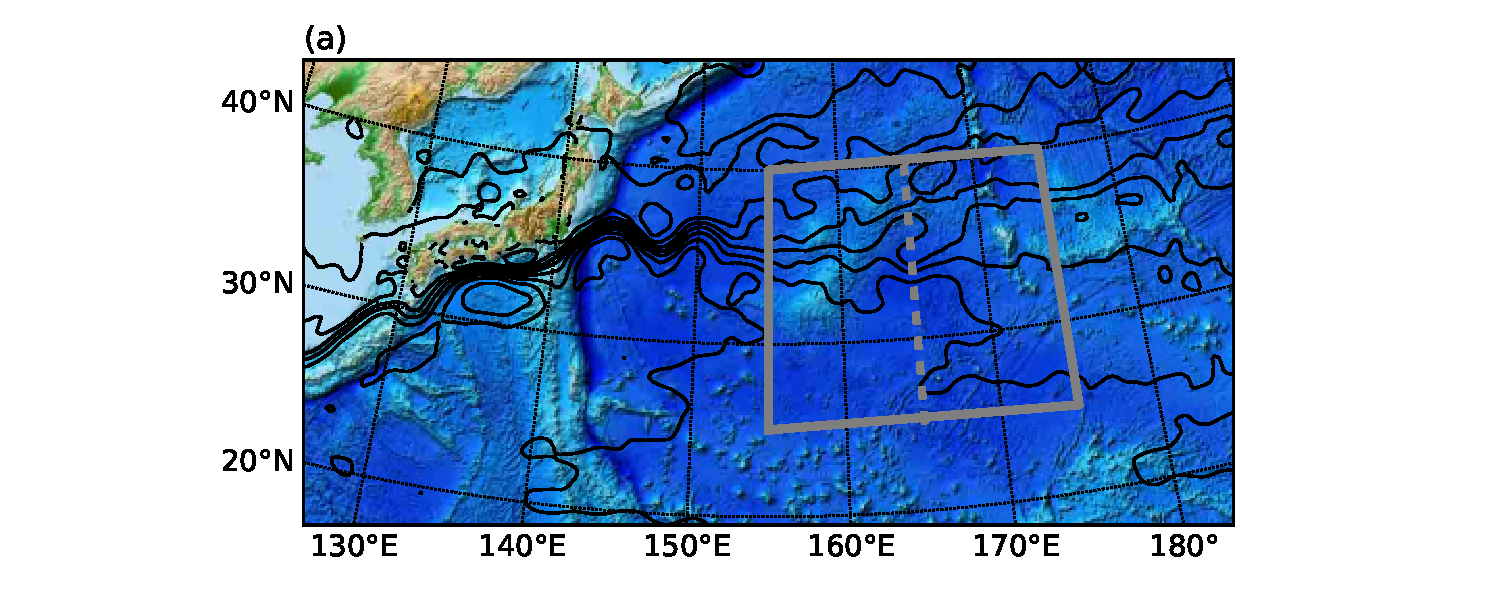
\includegraphics[width=.75\textwidth]{figs/fig1_1.pdf}\\
\vspace{-.125cm}
\includegraphics[width=.75\textwidth]{figs/fig1_2.pdf}
 \caption{(a) The study region with the subregion where the LLC outputs are
          analyzed. Colors represent the topography and white lines are contours of absolute
          dynamic topography every 0.1 m from AVISO. LLC 4320 (1/48$^\circ$) snapshots of surface vorticity (b and c) and transects
          of potential density at 165$^\circ$E (d and e). The snapshots were
          taken at 00:00 UTC.}
\vspace{-1.5cm}
 \label{fig1}
 \end{center}
 \end{figure*}

\section{Statistics of the surface lateral velocity gradient tensor}
To study the seasonality in the surface velocity, we calculate the lateral velocity gradient tensor
\begin{equation}
\left[\begin{matrix} u_x & u_y\\ v_x&v_y \end{matrix}\right]
\end{equation}
using a centered
second-order finite difference scheme. We then diagnose
the vertical vorticity
\begin{equation}
\zeta \equiv v_x - u_y\, ,
\end{equation}
lateral rate of strain
\begin{equation}
  \alpha \equiv [(u_x-v_y)^2 + (u_y + v_x)^2]^{1/2}\,,\\
\end{equation}
and horizontal divergence
\begin{equation}
\delta \equiv u_x + v_y\, .
\end{equation}
These diagnostics highlight the submesoscale structures in the flow
\citep[e.g.,][]{capet_etal2008a,shcherbina_etal2013}.

Figures \ref{fig1}b-c show snapshots of vertical vorticity $\zeta$ in early spring
(April 15) and fall (October 15) in the LLC4320 (1/48$^\circ$) simulation.
The model solutions depict seasonality in vorticity: large values of
fine-grained vertical vorticity are observed in early spring with maximum
values as large as $4f$, where $f$ is
the local planetary vorticity, and root-mean-square (RMS) of about $0.4f$. In early
fall, the situation is the opposite: the vertical vorticity is relatively coarse-grained;
its local maximum and RMS are both smaller than $0.5f$.
Indeed, the vorticity and rate of strain are strongest in wintertime (Figure \ref{fig2}):
in both simulations, the RMS vorticity and strain rate are about twice as large in
late winter/early spring
than in late summer/early fall. Because the wintertime vorticity and strain rate
are dominated by the smallest scales in the flow (the KE spectrum is shallower than
a $-3$ power law in winter), increasing the resolution from
1/24$^\circ$ to 1/48$^\circ$ increases the wintertime RMS vorticity
and strain by about 40$\%$.

 \begin{figure*}[ht]
   \begin{center}
     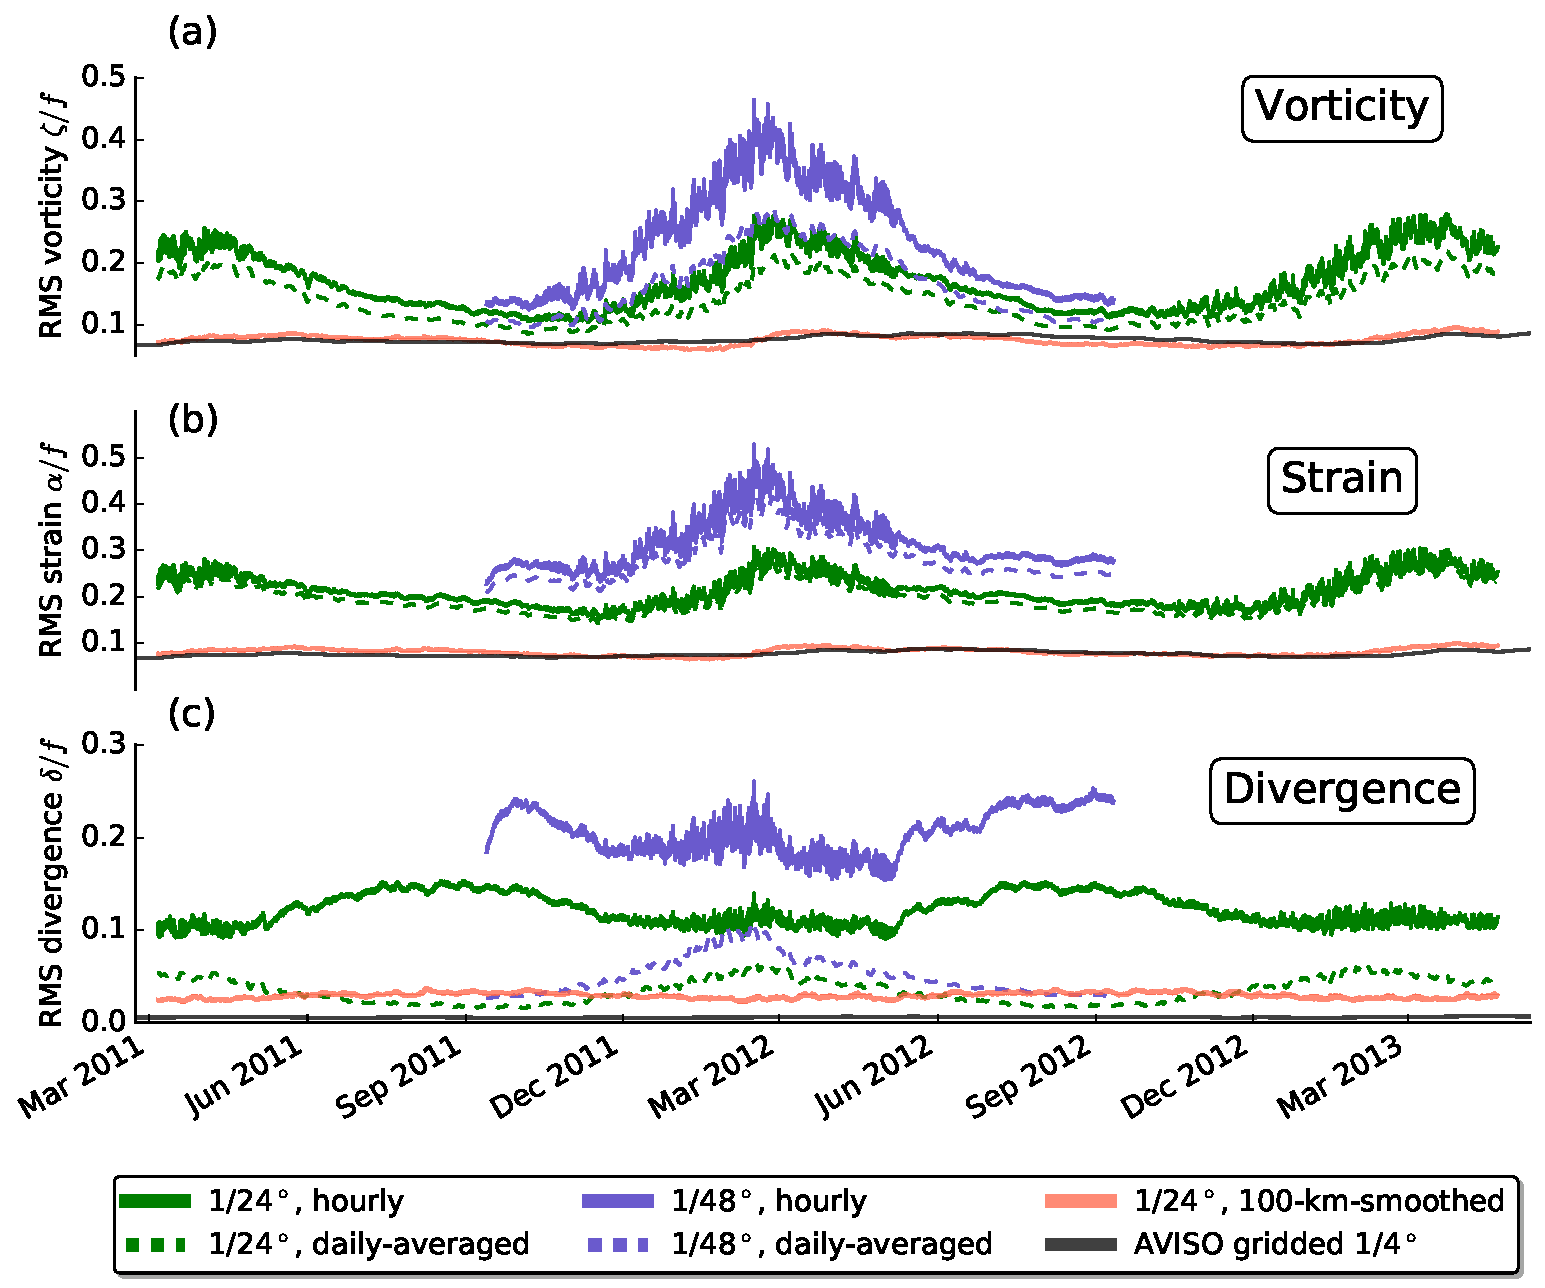
\includegraphics[width=.75\textwidth]{figs/fig2.pdf}
  \caption{Time series of the root-mean-square (RMS) of (a) vorticity,
  (b) rate of strain, and (c) horizontal divergence in the LLC outputs and gridded AVISO data.}
  \label{fig2}
  \end{center}
\end{figure*}

The bulk of vertical vorticity and strain rate are associated with subinertial flows
($T_f = 2\pi/f_0\approx 23.5$h, where $f_0$ is the inertial frequency at
the mean latitude): daily-averaging the velocity fields suppresses super-inertial
motions and reduces the RMS
vorticity by 40$\%$ and the RMS strain by 10$\%$; the seasonal
cycle remains strong (see
dashed lines in figures \ref{fig2}a-b). Indeed, most of this seasonal cycle is associated
with submesoscale flows: smoothing the velocity fields
with a Hanning filter with cut off scale of 100 km dramatically reduces the RMS
vorticity and strain rate. The reduction in variance is about 80$\%$ in winter,
yielding RMS vorticity and strain  rate roughly consistent with the diagnostics from
AVISO gridded geostrophic velocities (compare red lines to black lines in figures \ref{fig2}a-b).
The picture that emerges is consistent with recent studies: shallow baroclinic
instabilities energize the submesoscales in late winter, drawing from the available
potential energy stored in large lateral buoyancy gradients in deep mixed layers \citep{sasaki_etal2014,callies_etal2015,callies_etal2016}.

The seasonal cycle of the horizontal divergence, however, showcases the complexity
of the upper-ocean annual variability. If submesoscale eddies and fronts dominated
the near-surface variability all year, then the seasonal cycle of horizontal divergence,
vertical vorticity, and lateral strain rate would be in phase \citep[e.g.,][]{sasaki_etal2014}.
While there is a clear wintertime peak in divergence of daily-averaged velocity
(see dashed lines in figure \ref{fig2}c; RMS divergence $\sim0.1 f$ in the 1/48$^\circ$
simulation), the hourly fields show
a stronger enhancement of
lateral divergence in late summer/early fall (RMS divergence $\sim0.22 f$ the 1/48$^\circ$
simulation). Because the 1/48$^\circ$ simulation better resolves
smaller-scale submesoscale flows, a secondary RMS divergence peak in winter  is
nearly as strong as in summer. Submesoscale fronts and eddies evolve
relatively fast, and there is no clear
temporal and spatial scale separation between those motions and inertia-gravity waves
\citep{mcwilliams2016}:
daily-averaging the velocity fields efficiently suppresses the summertime horizontally
divergent flows, but also reduces the wintertime lateral divergence by about 50$\%$.
Figure \ref{fig2}c also shows that most of the lateral divergence is associated
with submesoscale flows: smoothing the velocity fields with a 100-km-cutoff
suppresses more than 80$\%$ of the RMS divergence.


\begin{figure*}[ht]
  \begin{center}
    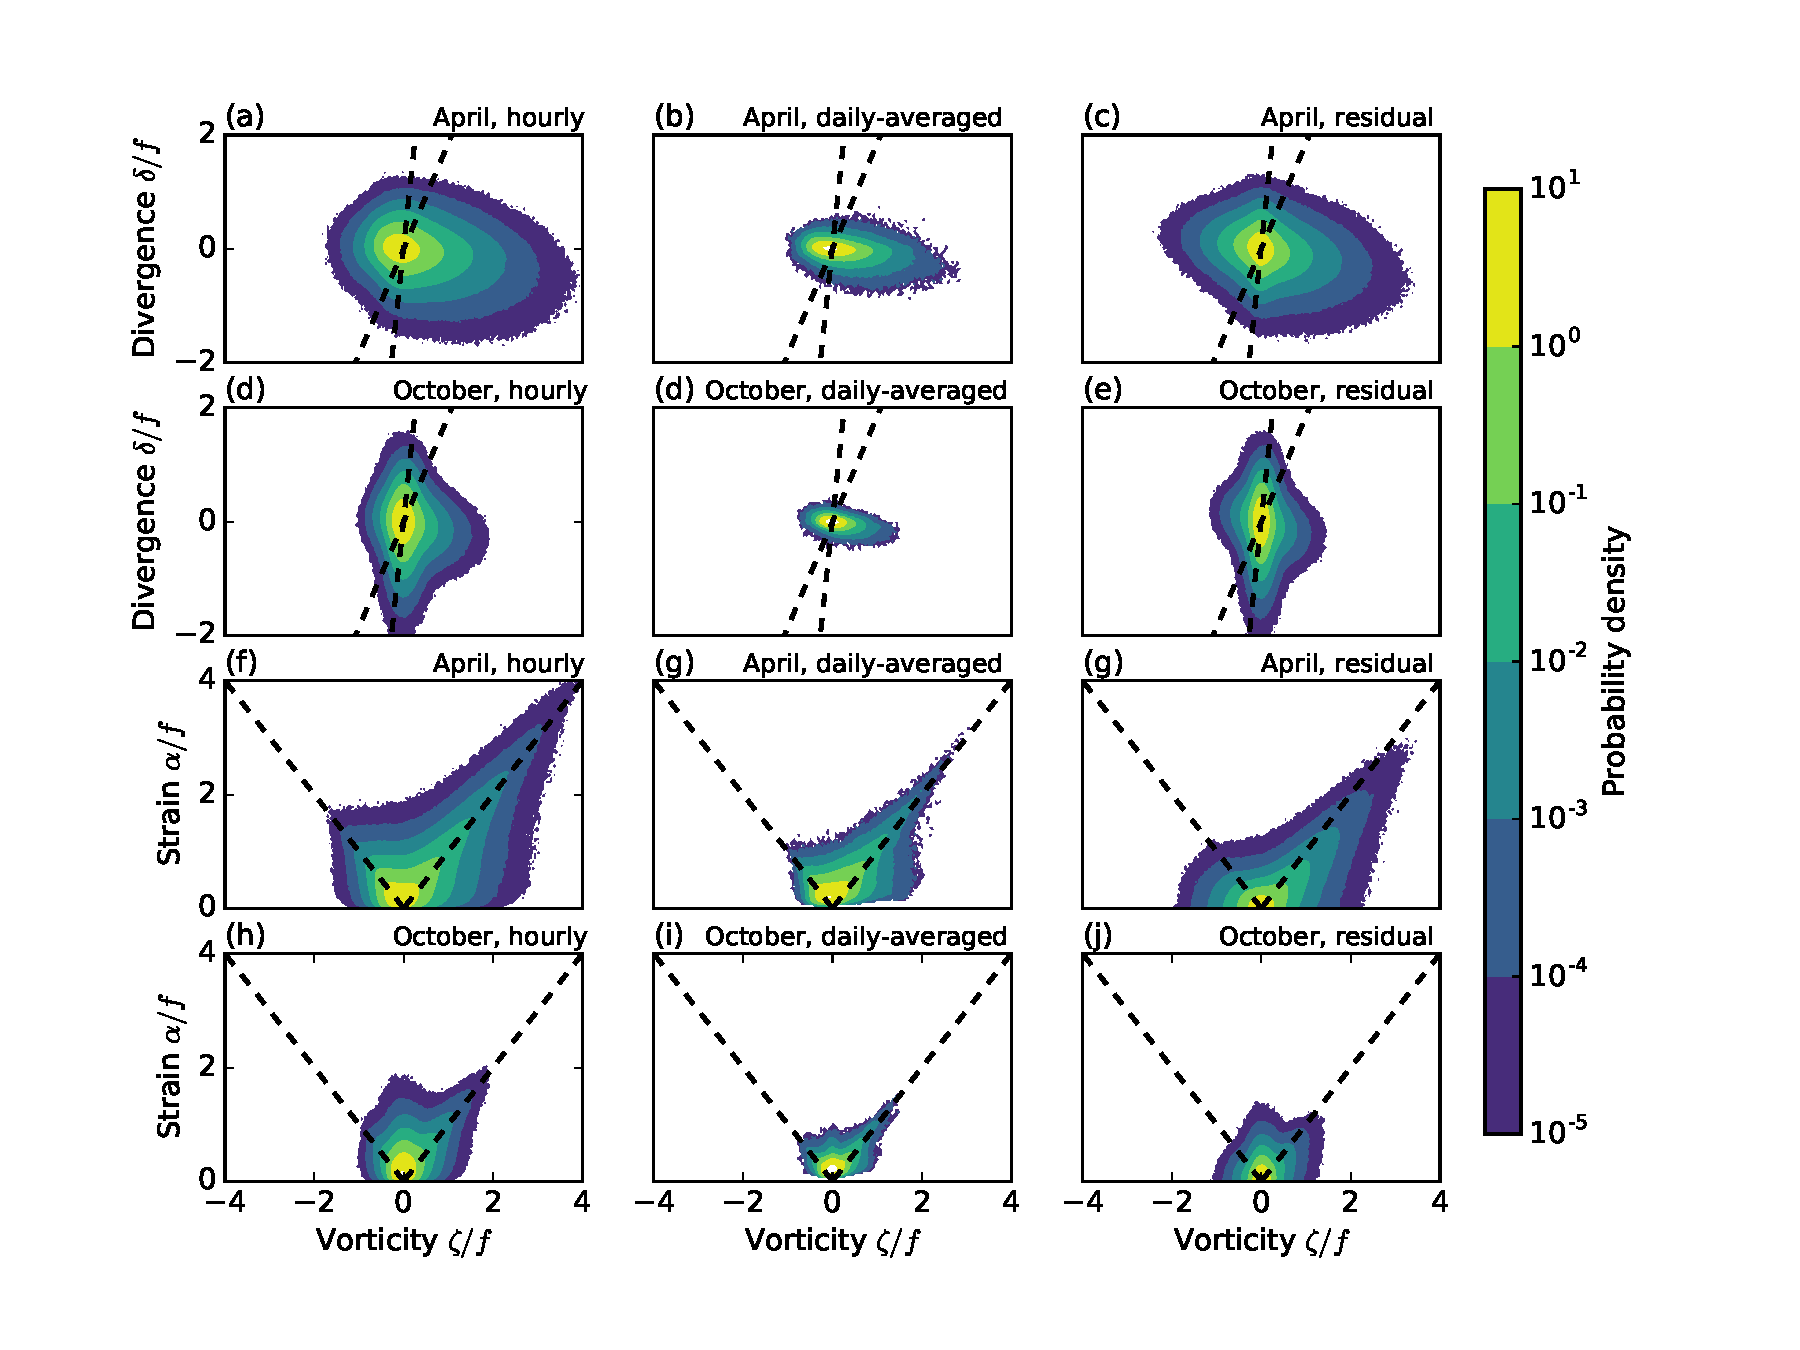
\includegraphics[width=.95\textwidth]{figs/fig3.pdf}
 \caption{Seasonal variation of joint probability distributions:  vorticity vs.\ strain rate (a through d),
          and vorticity vs.\ Laplacian of sea-surface height (e through h) in April (a, b,
          e, f) and October (c, d, g, h).
          Dashed lines in (a) through (d) represent one dimensional shear flow $\alpha = \pm\zeta$,
          characteristic of fronts. Dashed lines in (e) through
          (h) represent geostrophic flow $\zeta = \frac{g}{f}\nabla_h^2 \eta$.}
 \label{fig3}
 \end{center}
\end{figure*}

\section{Seasonality of submesoscale dynamics}
The results of figure \ref{fig2}a-c show that submesoscale surface
 variability stems from different dynamics in summer than in winter.
 To characterize these differences, we calculate
joint probability distributions (jPDF) of
vorticity-strain and vorticity-Laplacian of sea-surface height (Figure \ref{fig3}).

The April vorticity-strain joint-PDF has a shape characteristic of submesoscale turbulence
 (Figures \ref{fig3}a-b). The alignment of vorticity and strain $\alpha \sim \pm\zeta$
 with strong positive skewness are fingerprints of submesoscale fronts
 \citep{shcherbina_etal2013,mcwilliams2016}. The shape of the vorticity-strain
 jPDF is similar for hourly and daily-averaged fields, although
 the vorticity skewness reduces from 1.4 to 1.13 from hourly to daily-averaged.
 The April results are characteristic of winter, indicating that wintertime submesoscale
 surface velocity is strongly dominated by submesoscale turbulence.
 The hourly velocity and sea-surface heigh fields have an important
ageostrophic component as depicted by the jPDF of vorticity-Laplacian of SSH
winter (Figure \ref{fig3}e). In other words, even in April, when submesoscale turbulence
prevails, only the daily-averaged fields
are largely
in  geostrophic balance (the jPDF of daily-averaged vorticity vs.\\ Laplacian of sea-surface height
is an ellipse with large eccentricity and main axis tilted by 45$^\circ$; Figure \ref{fig3}f).

The October vorticity-strain jPDF shows much weaker skewness (the vorticity skewness
is 0.68 and 0.67 for hourly and daily-averaged velocities). The shape of the
vorticity-strain jPDF  appears to be a combination of two half-ellipses centered
about $\zeta=0$, one with a 45$^\circ$ slope (characteristic of submesocale fronts
that persist in summer) and one with a very steep slope.
That the submesoscale dynamics in October are mainly ageostrophic is clearly depicted
in the shape of jPDF of vorticity-Laplacian of sea-surface height for hourly fields
 (Figure \ref{fig3}g), which is an ellipse aligned in the vertical axis.
Daily-averaging the model suppresses the ageostrophic, super-inertial flows, and, therefore,
the daily-averaged flow is essentially geostrophic as depicted by the 45$^\circ$-tilted
ellipse in the vorticity-Laplacian of sea-surface height jPDF.

 Time series of PDFs of vorticity and divergence (supporting information) show
 a strong oscillation between these two regimes. In late winter/early spring
 the vorticity is strongly positively skewed, whereas the divergence is moderately
 negatively skewed as predicted by frontogenesis \citep[e.g., ][]{capet_etal2008a,mcwilliams2016}
. In late summer/early fall, the divergence is stronger, but PDFs are much less skewed,
consistent with linear inertia-gravity waves.

\section{Projection onto horizontal scales}

To better quantify the projection of these flows onto different horizontal
scales, we calculate wavenumber spectra of kinetic energy and sea-surface height
 variance.  Before calculating the spectra, time-mean and spatial linear
trends were removed, and the resulting fields were multiplied by a two-dimensional Hanning ``spectral window''.
The two-dimensional spectra were averaged azimuthaly \citep[e.g., ][]{rocha_etal2016} .
We discuss only spectra for the 1/48$^\circ$ simulation, which extends the 1/24$^\circ$ simulation
towards smaller scales (supporting information).



\begin{figure*}[ht]
  \begin{center}
    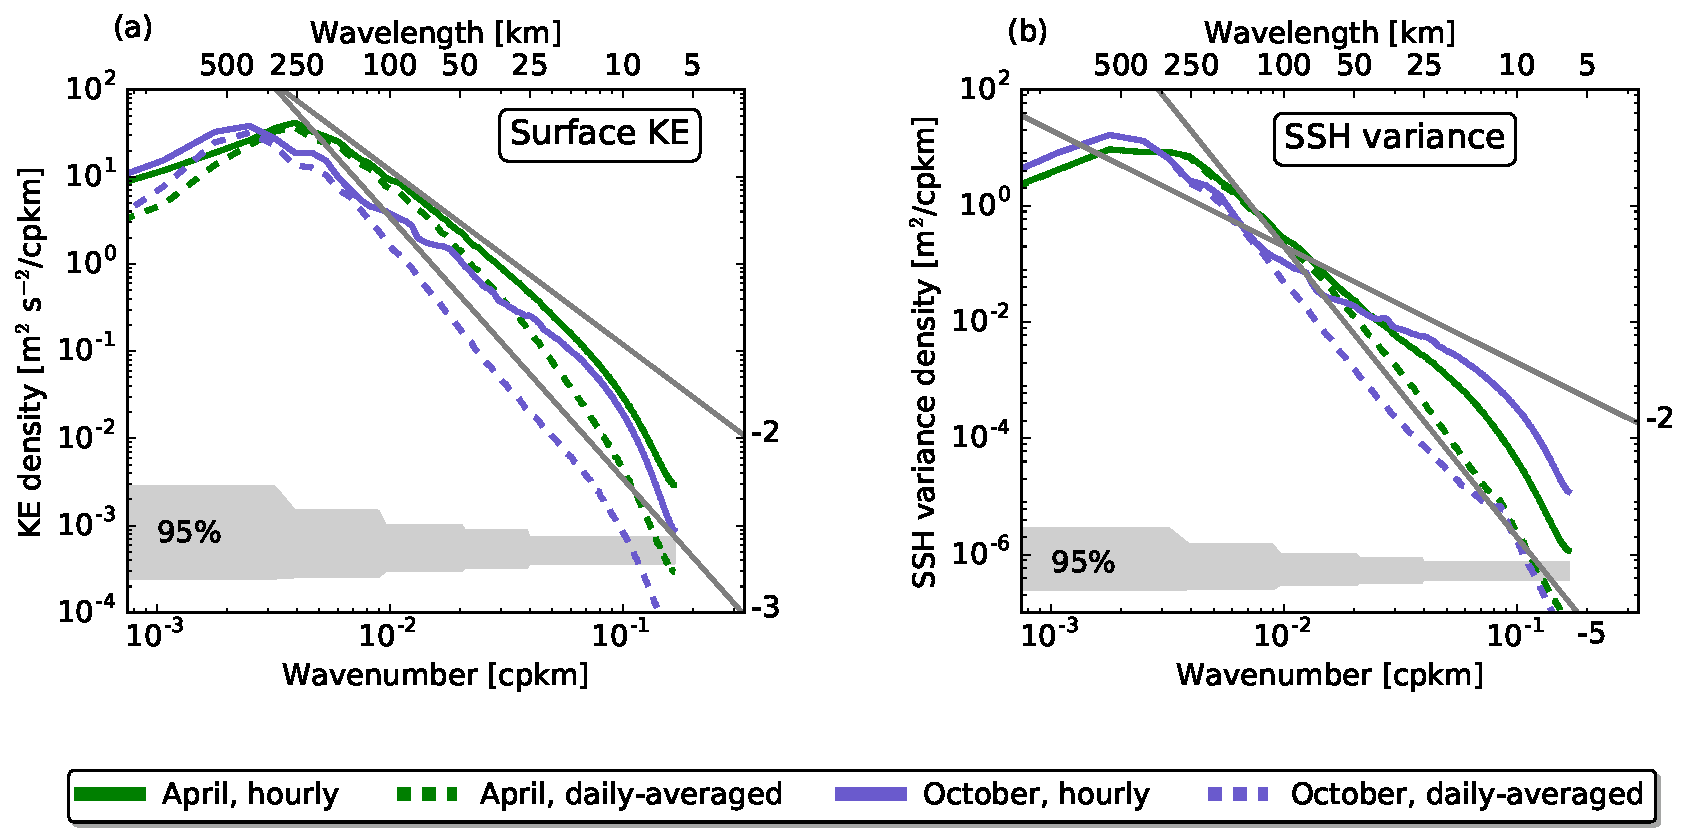
\includegraphics[width=1.\textwidth]{figs/fig4.pdf}
 \caption{Surface (horizontal) kinetic energy (a) and sea-surface height variance wavenumber spectra (b)
 in the 1/48$^\circ$ simulation. Solid lines
 are spectra based on hourly snapshots, and dashed lines are spectra based on daily-averaged
 fields.}
 \label{fig4}
 \end{center}
\end{figure*}


Figure \ref{fig4}a depicts the horizontal wavenumber spectra of surface KE in
April and October. At scales larger than 20 km, the April and October spectra based on hourly
velocity snapshots (solid lines) are nearly indistinguishable from each other within 95$\%$ confidence level.
Consistent with the results of
\citet{rocha_etal2016}, who analyzed a 3-month output of the LLC4320 simulation in Drake Passage,
there is significant high-frequency variabilty at submesoscales. Daily-averaging
the velocity field suppresses spatial variability at scales smaller than about 250
km, both in April and October (compare solid lines against dashed lines in Figure
\ref{fig4}a). But this suppression is dramatic in October, when the inertia-gravity waves peak. At scales
smaller than 100 km, 39$\%$ of the surface KE in April is accounted for by super-inertial
flows as opposed to 79$\%$ in October. The seasonality of subinertial submesoscale flows
is strong, consistent
with the results of \citet{sasaki_etal2014}, which are
based on daily-averaged velocity fields of a different model without tidal forcing
(P. Klein, personal communication).

The inertia-gravity waves project on the sea-surface.
There is a dramatic difference between the spectra
based on hourly and daily-averaged sea-surface height in October (Figure \ref{fig4}b): at scales smaller than 100 km, the spectra
of hourly sea-surface height roughly follows a $-2$ power-law, whereas the spectra of daily-averaged
sea-surface height roughly follows a $-5$ power-law. At these scales, 33$\%$ of the sea-surface height variance in April is accounted for by super-inertial
flows as opposed to 83$\%$ in October! Curiously, the out-of-phase seasonal cycle of submesoscale
turbulence and near-surface submesoscale inertia-gravity waves conspire to yield weak seasonality
in the spectra of KE and sea-surface height variance based on hourly fields.


\section{Summary and Conclusion}
Our work adds to recent modeling \citep{sasaki_etal2014}
and observational \citep{callies_etal2015,buckingham_etal2016} evidence of vigorous seasonality in
submesoscale turbulence. In particular, our main finding is that in global simulations with embedded tides the
near-surface submesoscale inertia-gravity waves in the Kuroshio Extension undergo
a strong seasonal cycle that is out of phase with the seasonal cycle of
submesoscale turbulence. We conjecture that the summertime dominance of inertia-gravity waves
 \citep{callies_etal2015} is a consequence both of suppression of submesoscale turbulence and
enhancement of inertia-gravity waves due to re-stratification of
the upper ocean.

\cite{dasaro1978} showed that the velocity of linear internal waves
in the mixed layer strongly depends on the density jump at the mixed layer
base, with largest mixed layer velocities when the jump is strongest.
In summer, the shallow mixed layer overlays a strong seasonal pycnocline,
and thus the internal waves projection onto the mixed layer may be stronger
according to \cite{dasaro1978}'s arguments. An
alternative explanation is that the shape of the baroclinic modes
changes seasonally. In particular the baroclinic modes are
significantly more surface intensified in late summer/early fall
 (supporting information).
If the internal wave source has weak seasonal dependence, then a strong
seasonal cycle in the near-surface expression of internal waves is expected.
Internal tide generation does not show a seasonal modulation \citep[e.g.,][]{alford2003},
and therefore one expects a strong seasonality in the near-surface
expression of internal tides and
other submesoscale inertia-gravity waves generated through internal tide interactions.
Near-inertial wave generation peaks in winter \citep[e.g.,][]{alford2003}, but
those waves project onto large horizontal scales \citep[e.g, ][]{qi_etal1995}.

An important caveat is that this study focuses on a single patch of ocean in the
vicinity of the Kuroshio Extension. This may be typical of a mesoscale-rich
subtropical region, but it is unlikely to be
representative of other regions such as low-eddy-kinetic-energy eastern boundary currents
and the middle of the subtropical gyre.  We plan to report on the geographic variability of submesoscale
 seasonality in a future study.

%The effects of smaller-scale/higher-frequency
%``sub-submesoscale'' flows on the submesoscale surface velocity and SSH variability
%are presently unknown.

% That the  surface velocity and SSH submesoscale variability may be
% dominated by ageostrophic flows in
% summer/fall has consequences for the interpretation of data from
% the future SWOT and COMPIRA altimeter missions,
% which will deliver SSH measurements at submesoscales. To the extent that
% high-frequency flows are dominated by spatially incoherent internal tides and other
% internal waves, it may be very difficult (if not impossible) to
% separate SSH submesoscale variability associated with geostrophic motions
% from high-frequency, ageostrophic flows. Thus, previous claims that
% one will be able to easily obtain submesoscale surface
% geostrophic velocities and monitor such seasonal cycle on global scales
% \citep{sasaki_etal2014,qiu_etal2014} are overstated.




% Here we argue that those divergent motions are likely inertia-gravity waves.
% We can show a couple of spectra and argue that they roughly satisfy polarization
% relations.
%
% We can also try and show some observations here. Any cruises with ADCP data.
% While it may be hard to have enough data for the errorbars to be small, a
% rough consistency may be better than nothing.
%
% Perhaps a mooring data should show strong seasonal modulation at high-frequencies?
%
% We must be able to present some observational evidence that the model is not
% misleading at high-frequencies.


% Here we argue that high-frequency (supra-daily) flows significantly project
% on the sea-surface, and thus estimation of submesoscale (10-100 km) geostrophic
% velocity from sea-surface height (SSH) is not warranted. Calculating spectral
% KE fluxes from both velocity and geostrophic velocity (from SSH) would
% contrast with the results in Sasaki et al.

% \section{Projection on time scales}
% To better understand the high-frequency/high-wavenumber flows  we calculate frequency
% spectra of surface KE winter \ref{fig4}). To obtain statistically meaningful results,
% we average spectral estimates along a section at 165$^\circ$E.  There is about 50
% independent spectral realizations.
%
% The surface KE spectra of subinertial flows very roughly follow a $-2$ power-law.
% The high-frequency flows are split near-inertial flows, tidal signals and their
% higher harmonics. Hence these high-frequency flows are dominated by inertia-gravity
% waves. (Note that the inertial peak nearly merges with the
% diurnal tide peak.) There is statistically significant seasonality. The seasonal
% cycle of the sub-inertial motions (at least for periods between 5-20 days)
% is out-of-phase with the seasonal cycle of supra-inertial flows: the former flows
% are more energetic in April and the latter in October.
%
% Most of these high-frequency inertia-gravity waves project onto scales smaller
% than 100 km. The surface KE spectra of 100-km-smoothed velocity field is significantly
% suppressed in supra-inertial frequencies --- there are no statistically significant
% changes at sub-inertial frequencies (see dashed lines in figure \ref{fig4}).

% say something about relative energy in smoother vs.\\ unsmoothed fields.
% also say something about comparison with observations.

%\begin{figure}[ht]
%  \begin{center}
%    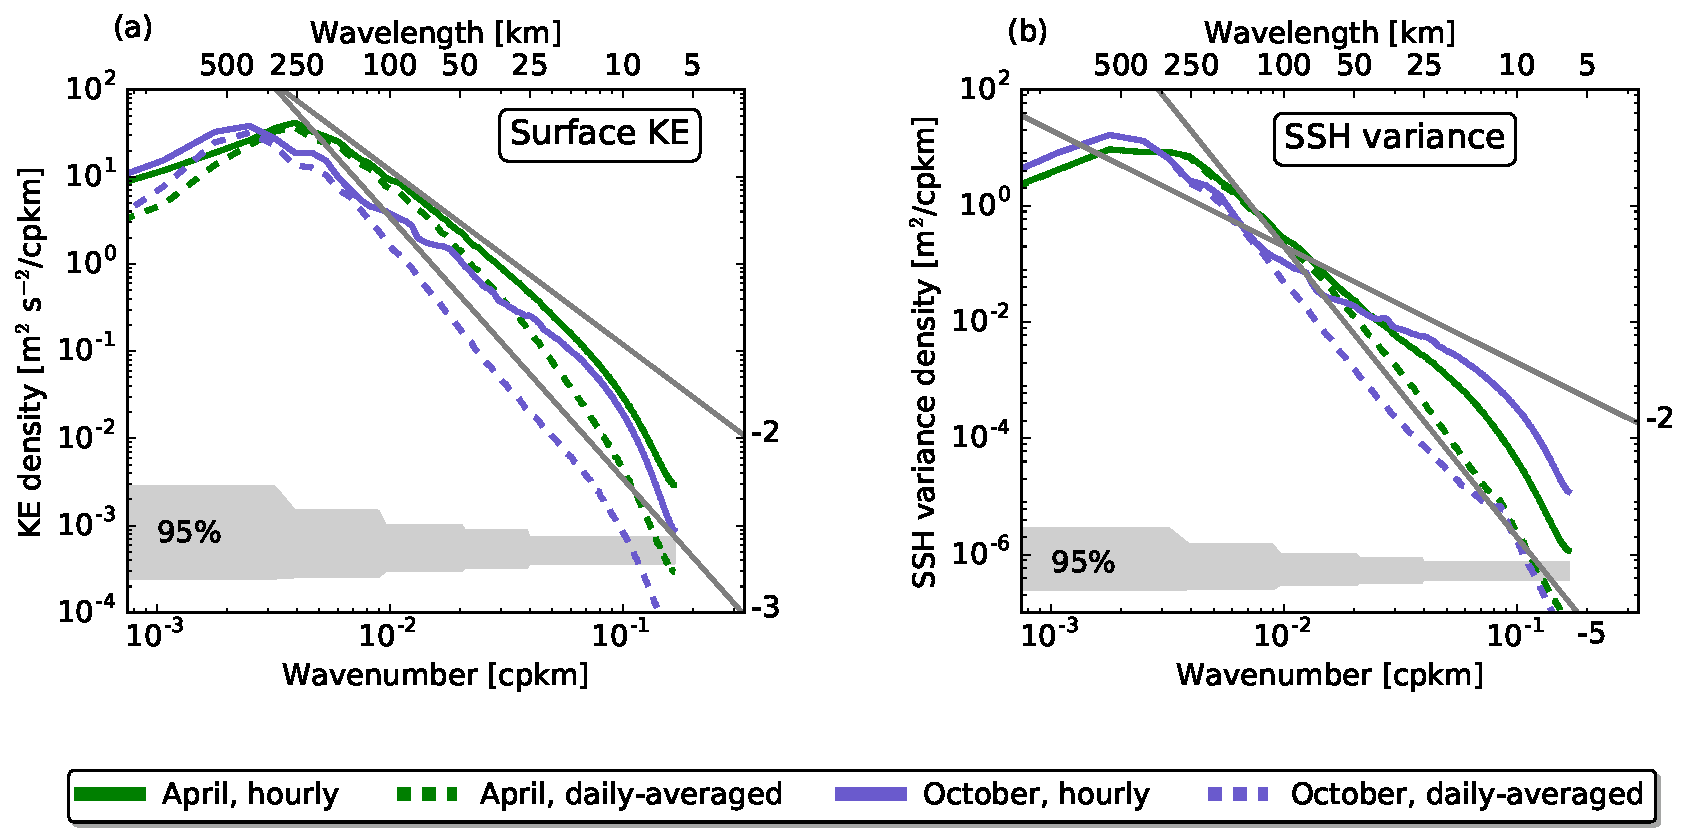
\includegraphics[width=.45\textwidth]{figs/fig4.pdf}
% \caption{Surface (horizontal) KE frequency spectra. Solid lines
% are spectra based on the 1/24$^\circ$ fields, dashed line are spectra
% based on 100-km-smoothed fields.}
% \label{fig4}
% \end{center}
%\end{figure}


%
%  ACKNOWLEDGMENTS

\begin{acknowledgments}
 William R. Young and the referees --- Christian Buckingham and two anonymous ---
  provided constructive and helpful comments. Greg Wagner first
 suggested that the near-surface shape of the baroclinic modes may change seasonally.
 We thank the MITgcm community and our colleagues at the NASA Advanced
Supercomputing (NAS) Division for their awesome support.
This research was funded by NSF (OCE1357047) and NASA (NNX13AE44G,NNX13AE85G,NNX16AH67G).
The LLC output can be obtained from the ECCO project (\texttt{http://ecco2.org/llc$\_$hires}). The altimeter products were produced by Ssalto/Duacs
and distributed by AVISO, with support from CNES (\texttt{http://www.aviso.altimetry.fr/duacs/}).
Codes and output files are available online at the project repository
 (\texttt{https://github.com/crocha700/UpperOceanSeasonality}).
\end{acknowledgments}

\bibliographystyle{agufull08}
%\bibliography{rocha_etal}



%  this should go in a supplementary material
%\clearpage

%\section{Supplemental material 1: Spectral errors}



%%% End of body of article:
%%%%%%%%%%%%%%%%%%%%%%%%%%%%%%%%
%% Optional Appendix goes here
%
% \appendix resets counters and redefines section heads
% but doesn't print anything.
% After typing \appendix
%
%\section{Here Is Appendix Title}
% will show
% Appendix A: Here Is Appendix Title
%
%%%%%%%%%%%%%%%%%%%%%%%%%%%%%%%%%%%%%%%%%%%%%%%%%%%%%%%%%%%%%%%%
%
% Optional Glossary or Notation section, goes here
%
%%%%%%%%%%%%%%
% Glossary is only allowed in Reviews of Geophysics
% \section*{Glossary}
% \paragraph{Term}
% Term Definition here
%
%%%%%%%%%%%%%%
% Notation -- End each entry with a period.
% \begin{notation}
% Term & definition.\\
% Second term & second definition.\\
% \end{notation}
%%%%%%%%%%%%%%%%%%%%%%%%%%%%%%%%%%%%%%%%%%%%%%%%%%%%%%%%%%%%%%%%


%% ------------------------------------------------------------------------ %%
%%  REFERENCE LIST AND TEXT CITATIONS
%
% Either type in your references using
% \begin{thebibliography}{}
% \bibitem{}
% Text
\begin{thebibliography}{18}
\providecommand{\natexlab}[1]{#1}
\expandafter\ifx\csname urlstyle\endcsname\relax
  \providecommand{\doi}[1]{doi:\discretionary{}{}{}#1}\else
  \providecommand{\doi}{doi:\discretionary{}{}{}\begingroup
  \urlstyle{rm}\Url}\fi

\bibitem[{\textit{Alford}(2003)}]{alford2003}
Alford, M.~H. (2003), {Redistribution of energy available for ocean mixing by
  long-range propagation of internal wave}, \textit{Nature},
  \textit{423}(6936), 159--162.

\bibitem[{\textit{Buckingham et~al.}(2016)\textit{Buckingham, Naveira~Garabato,
  Thompson, Brannigan, Lazar, Marshall, George~Nurser, Damerell, Heywood, and
  Belcher}}]{buckingham_etal2016}
Buckingham, C.~E., A.~C. Naveira~Garabato, A.~F. Thompson, L.~Brannigan,
  A.~Lazar, D.~P. Marshall, A.~George~Nurser, G.~Damerell, K.~J. Heywood, and
  S.~E. Belcher (2016), {Seasonality of submesoscale flows in the ocean surface
  boundary layer}, \textit{Geophysical Research Letters}, \textit{43}(5),
  2118--2126.

\bibitem[{\textit{B{\"u}hler et~al.}(2014)\textit{B{\"u}hler, Callies, and
  Ferrari}}]{buhler_etal2014}
B{\"u}hler, O., J.~Callies, and R.~Ferrari (2014), {Wave--vortex decomposition
  of one-dimensional ship-track data}, \textit{Journal of Fluid Mechanics},
  \textit{756}, 1007--1026.

\bibitem[{\textit{Callies et~al.}(2015)\textit{Callies, Ferrari, Klymak, and
  Gula}}]{callies_etal2015}
Callies, J., R.~Ferrari, J.~M. Klymak, and J.~Gula (2015), {Seasonality in
  submesoscale turbulence}, \textit{Nature communications}, \textit{6}.

\bibitem[{\textit{Callies et~al.}(2016)\textit{Callies, Flierl, Ferrari, and
  Fox-Kemper}}]{callies_etal2016}
Callies, J., G.~Flierl, R.~Ferrari, and B.~Fox-Kemper (2016), {The role of
  mixed-layer instabilities in submesoscale turbulence}, \textit{Journal of
  Fluid Mechanics}, \textit{788}, 5--41.

\bibitem[{\textit{Capet et~al.}(2008)\textit{Capet, McWilliams, Molemaker, and
  Shchepetkin}}]{capet_etal2008a}
Capet, X., J.~C. McWilliams, M.~J. Molemaker, and A.~Shchepetkin (2008),
  {Mesoscale to submesoscale transition in the California Current System. Part
  I: Flow structure, eddy flux, and observational tests}, \textit{Journal of
  Physical Oceanography}, \textit{38}(1), 29--43.

\bibitem[{\textit{D'Asaro}(1978)}]{dasaro1978}
D'Asaro, E.~A. (1978), {Mixed layer velocities induced by internal wave},
  \textit{Journal of Geophysical Research: Oceans}, \textit{83}(C5),
  2437--2438.

\bibitem[{\textit{Forget et~al.}(2015)\textit{Forget, Campin, Heimbach, Hill,
  Ponte, and Wunsch}}]{forget_etal2015}
Forget, G., J.-M. Campin, P.~Heimbach, C.~Hill, R.~Ponte, and C.~Wunsch (2015),
  {ECCO version 4: an integrated framework for non-linear inverse modeling and
  global ocean state estimation}, \textit{Geosci. Model Dev.}, \textit{8},
  3071--3104.

  \bibitem[{\textit{Marshall et~al.}(1997)\textit{Marshall, Hill, Perelman, and
    Adcroft}}]{marshall_etal1997}
  Marshall, J., C.~Hill, L.~Perelman, and A.~Adcroft (1997), Hydrostatic,
    quasi-hydrostatic, and nonhydrostatic ocean modeling, \textit{Journal of
    Geophysical Research: Oceans}, \textit{102}(C3), 5733--5752.

  \bibitem[{\textit{McWilliams}(2016)}]{mcwilliams2016}
  McWilliams, J.~C. (2016), {Submesoscale currents in the ocean}, in
    \textit{Proc. R. Soc. A}, vol. 472, p. 20160117, The Royal Society.

  \bibitem[{\textit{Menemenlis et~al.}(2008)\textit{Menemenlis, Campin, Heimbach,
    Hill, Lee, Nguyen, Schodlok, and Zhang}}]{menemenlis_etal2008}
  Menemenlis, D., J.-M. Campin, P.~Heimbach, C.~Hill, T.~Lee, A.~Nguyen,
    M.~Schodlok, and H.~Zhang (2008), ECCO2: High resolution global ocean and sea
    ice data synthesis, \textit{Mercator Ocean Quarterly Newsletter},
    \textit{31}, 13--21.

\bibitem[{\textit{Qi et~al.}(1995)\textit{Qi, De~Szoeke, Paulson, and
  Eriksen}}]{qi_etal1995}
Qi, H., R.~A. De~Szoeke, C.~A. Paulson, and C.~C. Eriksen (1995), {The
  structure of near-inertial waves during ocean storms}, \textit{Journal of
  Physical Oceanography}, \textit{25}, 2853--2871.

\bibitem[{\textit{Qiu et~al.}(2014)\textit{Qiu, Chen, Klein, Sasaki, and
  Sasai}}]{qiu_etal2014}
Qiu, B., S.~Chen, P.~Klein, H.~Sasaki, and Y.~Sasai (2014), {Seasonal mesoscale
  and submesoscale eddy variability along the North Pacific Subtropical
  Countercurrent}, \textit{Journal of Physical Oceanography}, \textit{44}(12),
  3079--3098.

\bibitem[{\textit{Richman et~al.}(2012)\textit{Richman, Arbic, Shriver,
  Metzger, and Wallcraft}}]{richman_etal2012}
Richman, J.~G., B.~K. Arbic, J.~F. Shriver, E.~J. Metzger, and A.~J. Wallcraft
  (2012), {Inferring dynamics from the wavenumber spectra of an eddying global
  ocean model with embedded tides}, \textit{Journal of Geophysical Research:
  Oceans}, \textit{117}(C12).

\bibitem[{\textit{Rocha et~al.}(2016)\textit{Rocha, Chereskin, Gille, and
  Menemenlis}}]{rocha_etal2016}
Rocha, C.~B., T.~K. Chereskin, S.~T. Gille, and D.~Menemenlis (2016),
  {Mesoscale to submesoscale wavenumber spectra in Drake Passage},
  \textit{Journal of Physical Oceanography}, \textit{46}, 601--620.

\bibitem[{\textit{Sasaki et~al.}(2014)\textit{Sasaki, Klein, Qiu, and
  Sasai}}]{sasaki_etal2014}
Sasaki, H., P.~Klein, B.~Qiu, and Y.~Sasai (2014), {Impact of oceanic-scale
  interactions on the seasonal modulation of ocean dynamics by the atmosphere},
  \textit{Nature communications}, \textit{5}.

\bibitem[{\textit{Shcherbina et~al.}(2013)\textit{Shcherbina, D'Asaro, Lee,
  Klymak, Molemaker, and McWilliams}}]{shcherbina_etal2013}
Shcherbina, A.~Y., E.~A. D'Asaro, C.~M. Lee, J.~M. Klymak, M.~J. Molemaker, and
  J.~C. McWilliams (2013), {Statistics of vertical vorticity, divergence, and
  strain in a developed submesoscale turbulence field}, \textit{Geophysical
  Research Letters}, \textit{40}(17), 4706--4711.

\bibitem[{\textit{Thompson et~al.}(2016)\textit{Thompson, Lazar, Buckingham,
  Naveira~Garabato, Damerell, and Heywood}}]{thompson_etal2016}
Thompson, A.~F., A.~Lazar, C.~Buckingham, A.~C. Naveira~Garabato, G.~M.
  Damerell, and K.~J. Heywood (2016), {Open-ocean submesoscale motions: A full
  seasonal cycle of mixed layer instabilities from gliders}, \textit{Journal of
  Physical Oceanography}, \textit{46}(4), 1285--1307.

\end{thebibliography}


% Or,
%
% If you use BiBTeX for your references, please use the agufull08.bst file (available at % ftp://ftp.agu.org/journals/latex/journals/Manuscript-Preparation/) to produce your .bbl
% file and copy the contents into your paper here.
%
% Follow these steps:
% 1. Run LaTeX on your LaTeX file.
%
% 2. Make sure the bibliography style appears as \bibliographystyle{agufull08}. Run BiBTeX on your LaTeX
% file.
%
% 3. Open the new .bbl file containing the reference list and
%   copy all the contents into your LaTeX file here.
%
% 4. Comment out the old \bibliographystyle and \bibliography commands.
%
% 5. Run LaTeX on your new file before submitting.
%
% AGU does not want a .bib or a .bbl file. Please copy in the contents of your .bbl file here.

%\begin{thebibliography}{}

%\providecommand{\natexlab}[1]{#1}
%\expandafter\ifx\csname urlstyle\endcsname\relax
%  \providecommand{\doi}[1]{doi:\discretionary{}{}{}#1}\else
%  \providecommand{\doi}{doi:\discretionary{}{}{}\begingroup
%  \urlstyle{rm}\Url}\fi
%
%\bibitem[{\textit{Atkinson and Sloan}(1991)}]{AtkinsonSloan}
%Atkinson, K., and I.~Sloan (1991), The numerical solution of first-kind
%  logarithmic-kernel integral equations on smooth open arcs, \textit{Math.
%  Comp.}, \textit{56}(193), 119--139.
%
%\bibitem[{\textit{Colton and Kress}(1983)}]{ColtonKress1}
%Colton, D., and R.~Kress (1983), \textit{Integral Equation Methods in
%  Scattering Theory}, John Wiley, New York.
%
%\bibitem[{\textit{Hsiao et~al.}(1991)\textit{Hsiao, Stephan, and
%  Wendland}}]{StephanHsiao}
%Hsiao, G.~C., E.~P. Stephan, and W.~L. Wendland (1991), On the {D}irichlet
%  problem in elasticity for a domain exterior to an arc, \textit{J. Comput.
%  Appl. Math.}, \textit{34}(1), 1--19.
%
%\bibitem[{\textit{Lu and Ando}(2012)}]{LuAndo}
%Lu, P., and M.~Ando (2012), Difference of scattering geometrical optics
%  components and line integrals of currents in modified edge representation,
%  \textit{Radio Sci.}, \textit{47},  RS3007, \doi{10.1029/2011RS004899}.

%\end{thebibliography}

%Reference citation examples:

%...as shown by \textit{Kilby} [2008].
%...as shown by {\textit  {Lewin}} [1976], {\textit  {Carson}} [1986], {\textit  {Bartholdy and Billi}} [2002], and {\textit  {Rinaldi}} [2003].
%...has been shown [\textit{Kilby et al.}, 2008].
%...has been shown [{\textit  {Lewin}}, 1976; {\textit  {Carson}}, 1986; {\textit  {Bartholdy and Billi}}, 2002; {\textit  {Rinaldi}}, 2003].
%...has been shown [e.g., {\textit  {Lewin}}, 1976; {\textit  {Carson}}, 1986; {\textit  {Bartholdy and Billi}}, 2002; {\textit  {Rinaldi}}, 2003].

%...as shown by \citet{jskilby}.
%...as shown by \citet{lewin76}, \citet{carson86}, \citet{bartoldy02}, and \citet{rinaldi03}.
%...has been shown \citep{jskilbye}.
%...has been shown \citep{lewin76,carson86,bartoldy02,rinaldi03}.
%...has been shown \citep [e.g.,][]{lewin76,carson86,bartoldy02,rinaldi03}.
%
% Please use ONLY \citet and \citep for reference citations.
% DO NOT use other cite commands (e.g., \cite, \citeyear, \nocite, \citealp, etc.).

%% ------------------------------------------------------------------------ %%
%
%  END ARTICLE
%
%% ------------------------------------------------------------------------ %%
\end{article}
%
%
%% Enter Figures and Tables here:
%
% DO NOT USE \psfrag or \subfigure commands.
%
% Figure captions go below the figure.
% Table titles go above tables; all other caption information
%  should be placed in footnotes below the table.
%
%----------------
% EXAMPLE FIGURE
%
 %\begin{figure}
 %\noindent\includegraphics[width=20pc]{samplefigure.eps}
 %\caption{Caption text here}
 %\label{figure_label}
 %\end{figure}
%
% ---------------
% EXAMPLE TABLE
%
%\begin{table}
%\caption{Time of the Transition Between Phase 1 and Phase 2\tablenotemark{a}}
%\centering
%\begin{tabular}{l c}
%\hline
% Run  & Time (min)  \\
%\hline
%  $l1$  & 260   \\
%  $l2$  & 300   \\
%  $l3$  & 340   \\
%  $h1$  & 270   \\
%  $h2$  & 250   \\
%  $h3$  & 380   \\
%  $r1$  & 370   \\
%  $r2$  & 390   \\
%\hline
%\end{tabular}
%\tablenotetext{a}{Footnote text here.}
%\end{table}

% See below for how to make sideways figures or tables.

\end{document}

%%%%%%%%%%%%%%%%%%%%%%%%%%%%%%%%%%%%%%%%%%%%%%%%%%%%%%%%%%%%%%%

More Information and Advice:

%% ------------------------------------------------------------------------ %%
%
%  SECTION HEADS
%
%% ------------------------------------------------------------------------ %%

% Capitalize the first letter of each word (except for
% prepositions, conjunctions, and articles that are
% three or fewer letters).

% AGU follows standard outline style; therefore, there cannot be a section 1 without
% a section 2, or a section 2.3.1 without a section 2.3.2.
% Please make sure your section numbers are balanced.
% ---------------
% Level 1 head
%
% Use the \section{} command to identify level 1 heads;
% type the appropriate head wording between the curly
% brackets, as shown below.
%
%An example:
%\section{Level 1 Head: Introduction}
%
% ---------------
% Level 2 head
%
% Use the \subsection{} command to identify level 2 heads.
%An example:
%\subsection{Level 2 Head}
%
% ---------------
% Level 3 head
%
% Use the \subsubsection{} command to identify level 3 heads
%An example:
%\subsubsection{Level 3 Head}
%
%---------------
% Level 4 head
%
% Use the \subsubsubsection{} command to identify level 3 heads
% An example:
%\subsubsubsection{Level 4 Head} An example.
%
%% ------------------------------------------------------------------------ %%
%
%  IN-TEXT LISTS
%
%% ------------------------------------------------------------------------ %%
%
% Do not use bulleted lists; enumerated lists are okay.
% \begin{enumerate}
% \item
% \item
% \item
% \end{enumerate}
%
%% ------------------------------------------------------------------------ %%
%
%  EQUATIONS
%
%% ------------------------------------------------------------------------ %%

% Single-line equations are centered.
% Equation arrays will appear left-aligned.

Math coded inside display math mode \[ ...\]
 will not be numbered, e.g.,:
 \[ x^2=y^2 + z^2\]

 Math coded inside \begin{equation} and \end{equation} will
 be automatically numbered, e.g.,:
 \begin{equation}
 x^2=y^2 + z^2
 \end{equation}

% IF YOU HAVE MULTI-LINE EQUATIONS, PLEASE
% BREAK THE EQUATIONS INTO TWO OR MORE LINES
% OF SINGLE COLUMN WIDTH (20 pc, 8.3 cm)
% using double backslashes (\\).

% To create multiline equations, use the
% \begin{eqnarray} and \end{eqnarray} environment
% as demonstrated below.
\begin{eqnarray}
  x_{1} & = & (x - x_{0}) \cos \Theta \nonumber \\
        && + (y - y_{0}) \sin \Theta  \nonumber \\
  y_{1} & = & -(x - x_{0}) \sin \Theta \nonumber \\
        && + (y - y_{0}) \cos \Theta.
\end{eqnarray}

%If you don't want an equation number, use the star form:
%\begin{eqnarray*}...\end{eqnarray*}

% Break each line at a sign of operation
% (+, -, etc.) if possible, with the sign of operation
% on the new line.

% Indent second and subsequent lines to align with
% the first character following the equal sign on the
% first line.

% Use an \hspace{} command to insert horizontal space
% into your equation if necessary. Place an appropriate
% unit of measure between the curly braces, e.g.
% \hspace{1in}; you may have to experiment to achieve
% the correct amount of space.


%% ------------------------------------------------------------------------ %%
%
%  EQUATION NUMBERING: COUNTER
%
%% ------------------------------------------------------------------------ %%

% You may change equation numbering by resetting
% the equation counter or by explicitly numbering
% an equation.

% To explicitly number an equation, type \eqnum{}
% (with the desired number between the brackets)
% after the \begin{equation} or \begin{eqnarray}
% command.  The \eqnum{} command will affect only
% the equation it appears with; LaTeX will number
% any equations appearing later in the manuscript
% according to the equation counter.
%

% If you have a multiline equation that needs only
% one equation number, use a \nonumber command in
% front of the double backslashes (\\) as shown in
% the multiline equation above.

%% ------------------------------------------------------------------------ %%
%
%  SIDEWAYS FIGURE AND TABLE EXAMPLES
%
%% ------------------------------------------------------------------------ %%
%
% For tables and figures, add \usepackage{rotating} to the paper and add the rotating.sty file to the folder.
% AGU prefers the use of {sidewaystable} over {landscapetable} as it causes fewer problems.
%
% \begin{sidewaysfigure}
% \includegraphics[width=20pc]{samplefigure.eps}
% \caption{caption here}
% \label{label_here}
% \end{sidewaysfigure}
%
%
%
% \begin{sidewaystable}
% \caption{}
% \begin{tabular}
% Table layout here.
% \end{tabular}
% \end{sidewaystable}
%
%
